%%%%%%%%%%%%%%%%%%%%%%%%%%%%%%%%%%%%%%%%%
% Beamer Presentation
% LaTeX Template
% Version 1.0 (10/11/12)
%
% This template has been downloaded from:
% http://www.LaTeXTemplates.com
%
% License:
% CC BY-NC-SA 3.0 (http://creativecommons.org/licenses/by-nc-sa/3.0/)
%
%%%%%%%%%%%%%%%%%%%%%%%%%%%%%%%%%%%%%%%%%

%----------------------------------------------------------------------------------------
%	PACKAGES AND THEMES
%----------------------------------------------------------------------------------------

\documentclass{beamer}

\mode<presentation> {

% The Beamer class comes with a number of default slide themes
% which change the colors and layouts of slides. Below this is a list
% of all the themes, uncomment each in turn to see what they look like.

%\usetheme{default}
%\usetheme{AnnArbor}
%\usetheme{Antibes}
%\usetheme{Bergen}
%\usetheme{Berkeley}
%\usetheme{Berlin}
%\usetheme{Boadilla}
\usetheme{CambridgeUS}
%\usetheme{Copenhagen}
%\usetheme{Darmstadt}
%\usetheme{Dresden}
%\usetheme{Frankfurt}
%\usetheme{Goettingen}
%\usetheme{Hannover}
%\usetheme{Ilmenau}
%\usetheme{JuanLesPins}
%\usetheme{Luebeck}
%\usetheme{Madrid}
%\usetheme{Malmoe}
%\usetheme{Marburg}
%\usetheme{Montpellier}
%\usetheme{PaloAlto}
%\usetheme{Pittsburgh}
%\usetheme{Rochester}
%\usetheme{Singapore}
%\usetheme{Szeged}
%\usetheme{Warsaw}

% As well as themes, the Beamer class has a number of color themes
% for any slide theme. Uncomment each of these in turn to see how it
% changes the colors of your current slide theme.

%\usecolortheme{albatross}
%\usecolortheme{beaver}
%\usecolortheme{beetle}
%\usecolortheme{crane}
%\usecolortheme{dolphin}
%\usecolortheme{dove}
%\usecolortheme{fly}
%\usecolortheme{lily}
%\usecolortheme{orchid}
%\usecolortheme{rose}
%\usecolortheme{seagull}
\usecolortheme{seahorse}
%\usecolortheme{whale}
%\usecolortheme{wolverine}

%\setbeamertemplate{footline} % To remove the footer line in all slides uncomment this line
%\setbeamertemplate{footline}[page number] % To replace the footer line in all slides with a simple slide count uncomment this line

%\setbeamertemplate{navigation symbols}{} % To remove the navigation symbols from the bottom of all slides uncomment this line
}
\usepackage{amsmath}
\usepackage{graphicx} % Allows including images
\usepackage{booktabs} % Allows the use of \toprule, \midrule and \bottomrule in tables

%----------------------------------------------------------------------------------------
%	TITLE PAGE
%----------------------------------------------------------------------------------------

\title[Pascal GPU Architecture]{Pascal GPU Architecture} % The short title appears at the bottom of every slide, the full title is only on the title page

\author[A.Zamani]{A.Zamani\\[1mm]{\small Supervised by: Dr. Motamedi}} % Your name
\institute[AUT] % Your institution as it will appear on the bottom of every slide, may be shorthand to save space
{
Amirkabir University of Technology \\ % Your institution for the title page
}
\date[February 2018]{February 2018} % Date, can be changed to a custom date

\begin{document}

\begin{frame}
\titlepage % Print the title page as the first slide
\end{frame}

\begin{frame}
\frametitle{Outline} % Table of contents slide, comment this block out to remove it
\tableofcontents % Throughout your presentation, if you choose to use \section{} and \subsection{} commands, these will automatically be printed on this slide as an overview of your presentation
\end{frame}

%----------------------------------------------------------------------------------------
%	PRESENTATION SLIDES
%----------------------------------------------------------------------------------------

%------------------------------------------------


\section{Introduction}
\begin{frame}
\frametitle{Introduction}
\begin{itemize}
	\item Graphic Processor Unit(GPU)
	\begin{itemize}
		\item {Games}
		\item {Graphical softwares}
			\begin{itemize}
				\item{Photoshop}
				\item{corel}
			\end{itemize}
		\item {Deep learning and Artificial Intelligence}
	\end{itemize}
\end{itemize}
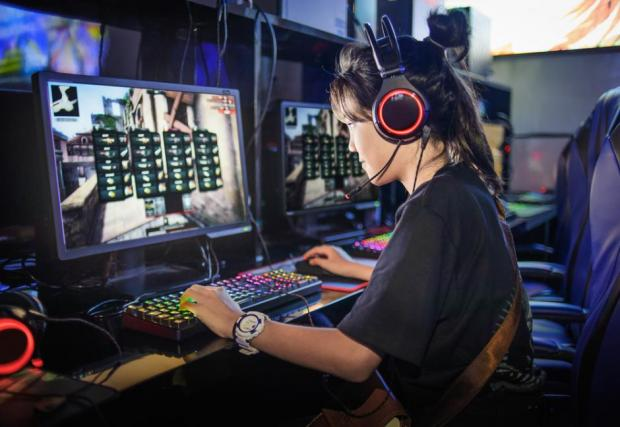
\includegraphics[scale=0.15]{game}

\includegraphics[scale=0.15]{Photoshop}
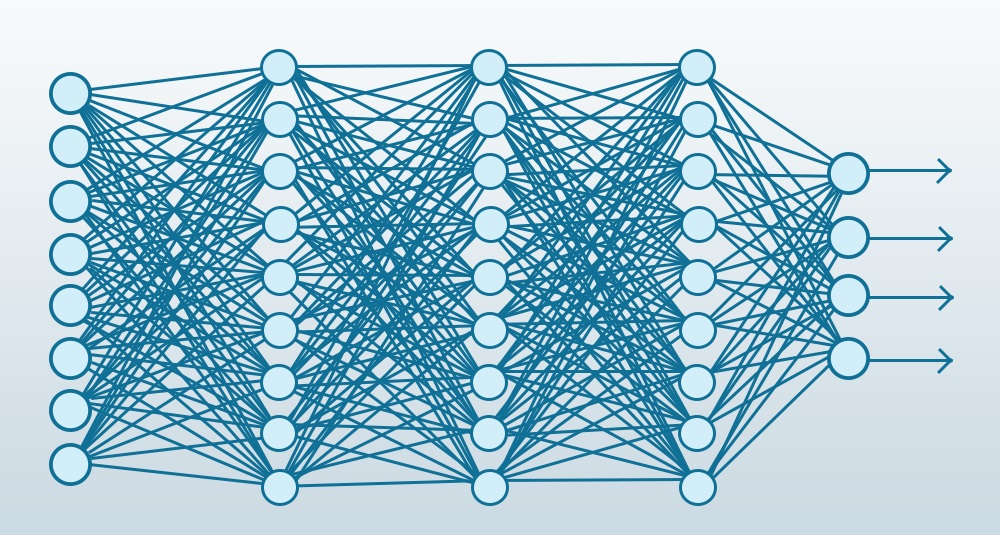
\includegraphics[scale=0.15]{deepLearning}
\begin{figure}
\centering

\includegraphics[scale=0.11]{corelDraw}

\end{figure}
\end{frame}
\begin{frame}
\frametitle{Introduction}
\begin{itemize}
	\item Nvidia
	\begin{itemize}
		\item {Pascal architecture}
		\item {Facebook and Google}
		\item {Audi and Benz - self drive}		
	\end{itemize}
\end{itemize}

\includegraphics[scale=0.3]{nvidia}
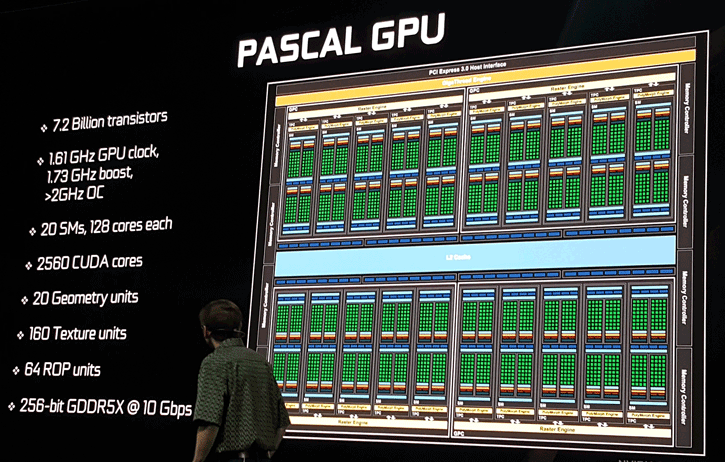
\includegraphics[scale=0.15]{pascal}

\includegraphics[scale=0.05]{Google-and-facebook}
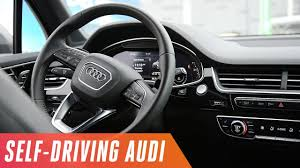
\includegraphics[scale=0.3]{Audi}
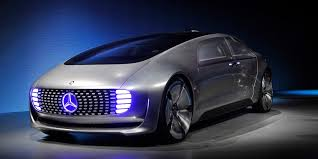
\includegraphics[scale=0.3]{Benz}
\end{frame}
\section{Graphic processing unit architecture}
\begin{frame}
	\frametitle{Graphics card}
	\begin{itemize}
		\item {First graphci card: IBM 1960 / 4 kb RAM / green}
		\item {Graphic Card Components}
		\begin{itemize}
			\item {Graphic processor: Main componet}
			\item {Memory}
			\item {Peripherals}
		\end{itemize}
	\end{itemize}
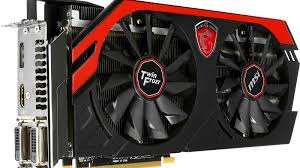
\includegraphics[scale=0.55]{graphiccard}

\includegraphics[scale=0.3]{ibm}
\end{frame}
\begin{frame}
\begin{itemize}
	\item {Vertex processor}
	\item {Pixel Fragment Processor}
\end{itemize}
\begin{itemize}
	\item Programming language
	\item NVidia 
	\item CUDA
\end{itemize}

\includegraphics[scale=0.3]{cuda}
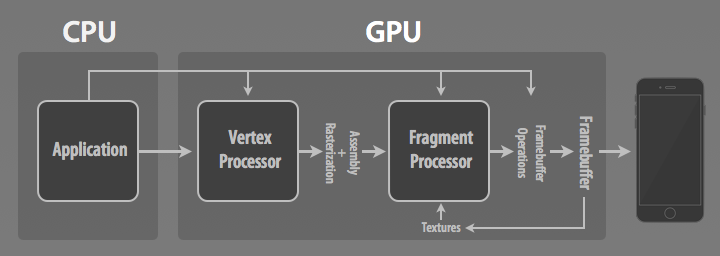
\includegraphics[scale=0.3]{vertex}
\end{frame}

\begin{frame}
\frametitle{CUDA}
\end{frame}

\begin{frame}
\frametitle{References}
[7] Drãxler, S., H. Karl, and Z.Á. Mann. Joint Optimization of Scaling and
Placement of Virtual Network Services. in 2017 17th IEEE/ACM
International Symposium on Cluster, Cloud and Grid Computing
(CCGRID). 2017.\\
$[8]$ Huin, N., B. Jaumard, and F. Giroire, Optimal Network Service Chain
Provisioning. IEEE/ACM Transactions on Networking, 2018. 26(3): p.
1320-1333.\\
$[9]$ Masri, W., et al. Minimizing delay in IoT systems through collaborative
fog-to-fog (F2F) communication. in 2017 Ninth International
Conference on Ubiquitous and Future Networks (ICUFN). 2017\\
$[10]$ Fan, J., et al. Deadline-Aware Task Scheduling in a Tiered IoT.Infrastructure. in GLOBECOM 2017 - 2017 IEEE Global Communications Conference. 2017.\\
$[11]$ Gupta, A., et al. Service Chain (SC) Mapping with Multiple SC
Instances in a Wide Area Network. in GLOBECOM 2017 - 2017 IEEE
Global Communications Conference. 2017.
\end{frame}
\begin{frame}
	
\begin{figure}
	\centering
	
\includegraphics[width=0.7\linewidth]{thanks}
		\label{fig:thanks}
\end{figure}
\end{frame}
\end{document} 